\section{Relational cross-attention and the abstractor module}\label{sec:abstractor_module}

At a high level, the primary function of an Abstractor is to compute abstract relational features of its inputs.\footnote{In this paper, we will use the name `Abstractor' to refer to both the module and to model architectures which contain the Abstractor module as a main component.} That is, given a sequence of input objects $x_1, \ldots, x_\m$, the Abstractor learns to model a relation $r(\cdot, \cdot)$ and computes a function on the set of pairwise relations between objects ${\{ r(x_i, x_j) \}}_{ij}$. At the heart of the Abstractor module is an inductive bias we call the \textit{relational bottleneck}, that disentangles relational information from the features of individual objects.

\subsection{Modeling relations as inner products}\label{ssec:relations_as_inner_prods}

A ``relation function'' maps a pair of objects $x_1, x_2 \in \calX$ to a vector representing the relation between the two objects. We model pairwise relations as inner products between appropriately encoded (or `filtered') object representations. In particular, we model the pairwise relation function $r(\cdot, \cdot) \in \mathbb{R}^{d_r}$ in terms of $d_r$ learnable `left encoders' $\phi_1, \ldots, \phi_{d_r}$, and $d_r$ `right encoders' $\psi_1, \ldots, \psi_{d_r}$,
\begin{equation}\label{eq:inner_prod_rel}
    r(x_1,x_2) = \left(\langle \phi_1(x_1), \psi_1(x_2) \rangle, \langle \phi_2(x_1), \psi_2(x_2) \rangle, \ldots, \langle \phi_{d_r}(x_1), \psi_{d_r}(x_2) \rangle \right) \in \mathbb{R}^{d_r}.
\end{equation}
% A common choice is to model $(\phi_i, \psi_i)_{i\in [d_r]}$ as linear or affine maps. Considering all pairwise relations yields a \textit{relation tensor}, $R = \left[r(x_i, x_j)\right]_{i,j} \in \mathbb{R}^{\m \times \m \times d_r}$.

% AWNI: removed this for space. can add this back (or some version of it) if we think it's important. focusing on santoro1 for an entire paragraph might be distracting; although it does help explain the relational bottleneck. also worth noting, the current relconvnet paper has a similar paragraph.

% In principle, relations could be modeled by an arbitrary learnable function applied to the concatenation of the features of a pair of objects.~\citep{santoro1} takes this approach and models relations through MLPs applied to the concatenation of the features of a pair of objects. This approach is versatile in principle and can work given enough data. However, modeling relations as inner products has some important advantages. First, it induces a pressure on the resultant representations to encode relational information and constricts the leakage of information about individual objects. When relations are modeled as $g_\theta(\mathrm{concat}(x_1, x_2))$, for some parameterized function class $g_\theta$, there is no pressure or restriction that this function represents relations between the two objects---it can just as well represent information about the objects' features individually.

Modeling relations as inner products $\iprod{\phi(x_1)}{\psi(x_2)}$ ensures that the output represents a comparison between the two objects' features. More precisely, inner product relations induce a geometry on the object space $\calX$, since the inner product $\iprod{\phi(x_1)}{\phi(x_2)}$ induces well-defined notions of distance, angles, and orthogonality between objects in $\calX$. %Modeling relations as inner products is an approach that has been explored in previous work on relational architectures (e.g.,~\citep{esbn,kerg2022neural}) and has been shown to be a useful inductive bias on several discriminative relational tasks.
Considering all pairwise relations yields a \textit{relation tensor}, $R = \left[r(x_i, x_j)\right]_{i,j} \in \mathbb{R}^{\m \times \m \times d_r}$.
\subsection{Relational Cross-Attention}\label{ssec:relational_crossattention}

The core operation in a Transformer is attention. For an input sequence $X = \paren{x_1, \ldots, x_\m}$, self-attention transforms the sequence via, $ X' \gets \phi_v(X) \, \mathrm{Softmax}\paren{{\phi_q(X)}^\top \phi_k(X)}$,
% \begin{equation}\label{eq:self_attn}
%     X' \gets \phi_v(X) \, \mathrm{Softmax}\paren{\phi_q(X)^\top \phi_k(X)},
% \end{equation}
where $\phi_q, \phi_k, \phi_v$ are functions on $\calX$ applied independently to each object in the sequence (i.e., $\phi(X) = \paren{\phi(x_1), \ldots, \phi(x_\m)}$). Typically, those are linear or affine functions.
% , with $\phi_q, \phi_k$ having the same dimensionality so we can take their inner product. 
Note that $R := \phi_q(X)^\top \phi_k(X)$ is a relation matrix in the sense defined above. Self-attention admits an interpretation as a form of message-passing as follows, 
\begin{equation}\label{eq:self_attn_message_passing}
    x_i' \gets \mathrm{MessagePassing}\paren{\set{(\phi_v(x_j), R_{ij})}_{j \in [\m]}} = \sum_{j} R_{ij} \phi_v(x_j).
\end{equation}
where $m_{j \to i} = (\phi_v(x_j), R_{ij})$ is the message from object $j$ to object $i$, encoding the sender's features and the relation between the two objects, and $\bar{R} = \mathrm{Softmax}\paren{R}$ is the softmax-normalized relation matrix. Hence, the processed representation obtained by self-attention is an entangled mixture of relational information and object-level features.
% Thus, self-attention is a form of message-passing where the message from object $j$ to object $i$ is an encoding of object $j$'s features weighted by the (softmax-normalized) relation between the two objects. As a result, the processed representation obtained by self-attention involves some relational information. However, this relational information is entangled with object-level features.

Our goal is to learn relational representations which are abstracted away from object-level features in order to achieve more sample-efficient learning and improved generalization in relational reasoning. This is not naturally supported by the entangled representations produced by standard self-attention. We achieve this via a simple modification of attention---we replace the values $\phi_v(x_i)$ with vectors that \textit{identify} objects, but do not encode any information about their features. We call the vectors \textit{symbols}. Hence, the message sent from object $j$ to object $i$ is $m_{j \to i} = (s_j, R_{ij})$, the relation between the two objects, together with with the symbol identifying the sender object $j$,
\begin{equation}\label{eq:relational_crossattn_message_passing}
    A_i \gets \mathrm{MessagePassing}\paren{\set{(s_j, R_{ij})}_{j \in [\m]}} = \sum_{j} \bar{R}_{ij} s_j.
\end{equation}
Symbols act as abstract references to objects. They do not contain any information about the contents or features of the objects, but rather \textit{refer} to objects.
%  via their position. The symbols $S = (s_1, s_2, \ldots)$ can be either learned parameters of the model or nonparametric positional embeddings.
Suppose for now that each object $x_i$ is assigned a symbol $s_i$ in a manner that satisfies this property. We will discuss symbol-assignment mechanisms in the next subsection.
The vectors $\{s_i\}$ are `symbols' in the same sense that we call `$x$' a symbol in an equation like $y = x^2$---they are a reference to an object with an unspecified value. The difference is that the symbols here are `distributed representations' (i.e., vectors), leading to a novel perspective on the long-standing problem of neural versus symbolic computation.

This modification yields a variant of attention that we call \textit{relational cross-attention}, given by
\begin{equation}\label{eq:relational_crossattn}
    X' \gets S \, \sigma_{\mathrm{rel}}\paren{\phi(X)^\top \psi(X)},
\end{equation}
where $S = (s_1, \ldots, s_m)$ are the symbols, $\sigma_{\mathrm{rel}}$ is the relation activation function, and $\phi, \psi$ correspond to the query and key transformations. When the relation activation function $\sigma_{\mathrm{rel}}$ is softmax, this corresponds to $\mathrm{Attention}(Q \gets X,\, K \gets X,\, V \gets S)$. In contrast, self-attention corresponds to $\mathrm{Attention}(Q \gets X,\, K \gets X,\, V \gets X)$, mixing relational information with object-level features.

We observe in our experiments that allowing $\sigma_{\mathrm{rel}}$ to be a configurable hyperparameter can lead to performance benefits in some tasks. Softmax has the effect of normalizing the relation between a pair of objects $(i,j)$ based on the strength of $i$'s relations with the other objects in the sequence. In some tasks this is useful. In other tasks, this may mask relevant information, and element-wise activations (e.g., tanh, sigmoid, or linear) may be more appropriate.

Relational cross-attention implements a type of information bottleneck, which we term the relational bottleneck, wherein the resultant representation encodes only relational information about the object sequence (\Cref{fig:attn_mechanisms}) and does not encode information about the features of individual objects\footnote{The diagonal entries of the relation matrix $R_{ii} = \iprod{\phi(x_i)}{\psi(x_i)}$ encode information about individual objects. This can be interpreted as a leakage of non-relational information. It's possible to implement a stricter relational bottleneck by masking the diagonal entries of $R$, but we find this to be unnecessary in our experiments.}. This enables a branch of the model to focus purely on modeling the relations between objects, yielding greater sample-efficiency in tasks that rely on relational reasoning.

% \begin{remark}
%     We call this operation ``relational cross-attention'' because 1) it computes relational representations, and 2) when attending to the input objects,  only
%     relational information, not sensory information, is allowed to cross over, since 
%     the values are input-independent. \awni{I was thinking (1) explains `relational' and (2) explains `cross-attention'. But we might want to remove this since we're tight on space and it's not really necessary.}
% \end{remark}

In our experiments, $\phi_i, \psi_i$ are linear maps $W_1^{(i)}, W_2^{(i)}$, and relational cross-attention is given by
\begin{equation}
    \begin{split}
        \mathrm{RelationalCrossAttention}(X, S) &= \mathrm{MultiHeadAttention}\paren{Q \gets X,\, K \gets X,\, V \gets S} \\
        &= W_o \, \mathrm{concat}\paren{A^{(1)}, \ldots, A^{(d_r)}}, \\
        \text{where } A^{(i)} &= W_o^{(i)} S \, \sigma_{\mathrm{rel}}\paren{(W_1^{(i)} X)^\top (W_2^{(i)} X)}.
    \end{split}
\end{equation}

\begin{figure}
    \begin{subfigure}[b]{0.5\textwidth}
        \centering
        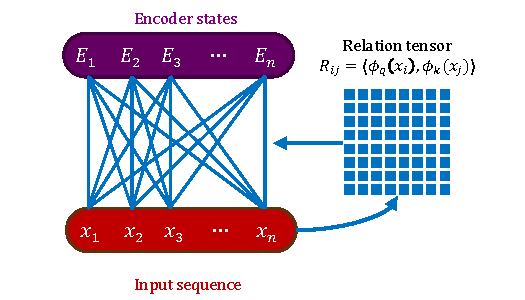
\includegraphics[width=\textwidth]{figures/self_attn_fig.pdf}
        \caption{$E \gets \mathrm{SelfAttention}(X)$}\label{fig:self_attention}
    \end{subfigure}
    \hfill
    \begin{subfigure}[b]{0.5\textwidth}
        \centering
        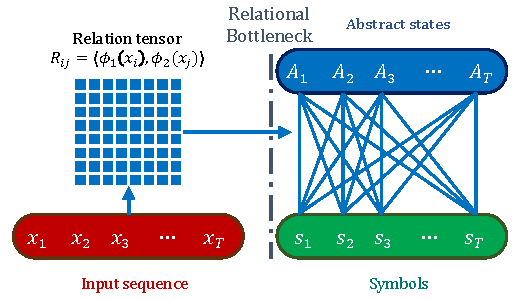
\includegraphics[width=\textwidth]{figures/rel_crossattn_fig.pdf}
        \caption{$A \gets \mathrm{RelationalCrossAttention(X, S)}$}\label{fig:relational_cross_attention}
    \end{subfigure}
    \caption{Comparison of relational cross-attention with self-attention. Red represents object-level features, blue represents relational features, and purple represents mixed representations. Relational cross-attention computes relational information disentangled from the features of individual objects.}\label{fig:attn_mechanisms}
    \vskip-10pt
\end{figure}

\subsection{Symbol assignment mechanisms}\label{ssec:symbol_assignment}
We propose three mechanisms of assigning symbols to objects. The key property that symbol assignment mechanisms must satisfy is to identify the object, without encoding its features.

\textbf{Positional symbols.} The simplest symbol assignment mechanism which satisfies this property is to simply assign each object a symbol based on the position it appears in the sequence. That is, we maintain a library of symbols $S_{\mathrm{lib}} = (s_1, \ldots, s_{\mathtt{max\_len}}) \in \reals^{d_s \times \mathtt{max\_len}}$, and we map the $i$-th object $x_i$ to the symbol $s_i$. While very simple, positional symbols are empirically certain tasks. $S_\mathrm{lib}$ can be either learned parameters of the model or nonparametric positional embeddings (e.g., sinusoidal).

\textbf{Position-relative symbols.} Similar to to position-relative embeddings, we can compute relational cross-attention with position-relative symbols via $A_i \gets \sum_j R_{ij} s_{j-i}$, where the symbol library is $S_{\mathrm{lib}} = \paren{\ldots, s_{-1}, s_0, s_1, \ldots}$.

\textbf{Symbolic attention.} We learn a library of symbols $S_{\mathrm{lib}} = (s_1, \ldots, s_{n_s}) \in \reals^{d_s \times n_s}$, where $n_s$ is the number of symbols in the library. For each object $x_i$, we retrieve a symbol by cross-attending to the symbol library, $s_i \gets \mathrm{CrossAttention}(x_i, S_{\mathrm{library}})$. Note that this weakens the relational bottleneck since object-level features are used to retrieve a symbol for each object. However, the dependence is only with respect to a low-dimensional projection of the object-level features, which we think of as encoding the object's ``syntactic role.'' Encoding such information in the symbols allows identifying objects by their role.

Ultimately, after relational cross-attention, the Abstractor state $A_i$ encodes the relations between object $i$ and each object $j$ in the sequence, identifying $j$ by its position, relative-position, or ``syntactic role,'' depending on the symbol-assignment mechanism used.

%TODO: add more in-depth discussion to appendix. including role of self-attention prior, in certain architectures, the strength of the relational bottleneck etc. Examples of what we think of "roles" in symbolic attention being.
\subsection{The Abstractor module}\label{ssec:abstractor_module}

We now describe the Abstractor module. Like the Encoder in a Transformer, this is a module that processes an input sequence of objects $X = \paren{x_1, \ldots, x_\m}$ producing a processed sequence of objects $A = \paren{A_1, \ldots, A_\m}$ that represents features of the input sequence. In an Encoder, the output objects represent a mix of object-level features and relational information. In an Abstractor, the output objects are abstract states that represent purely relational information, abstracted away from the features of individual objects. The core operation in an Abstractor module is relational cross-attention. Mirroring an Encoder, an Abstractor module can comprise several layers, each composed of relational cross-attention followed by a feedforward network. Optionally, residual connections and layer-normalization can be applied as suggested by~\citet{vaswani2017attention}. The algorithmic description is presented in~\Cref{alg:abstractor_module}.

\begin{algorithm}[ht!]
	\caption{Abstractor module}\label{alg:abstractor_module}
	\SetKwInOut{Input}{Input}
	% \SetKwInOut{Output}{Output}
	% \SetKwInOut{LearnableParams}{Learnable parameters}
	% \SetKwInOut{HyperParams}{Hyperparameters}

	\Input{object sequence: $\bm{X} = (x_1, \ldots, x_\m) \in \reals^{d \times \m}$ }
	% \HyperParams{Dimension of relation $d_r$, Projection dimension $d_p$, dimension of embedding $d_e$}
	% \LearnableParams{projection matrices $W_1^{(i)}, W_2^{(i)} \in \reals^{d_p \times d_e}, \ i=1, \ldots, d_r$, parameters of feedforward networks}
	\vspace{1em}

    $A^{(0)} \gets S_{1:\m}$

	\For{\(l \gets 1\) \KwTo \(L\)}{

        $A^{(l)} \gets \mathrm{RelationalCrossAttention}\paren{X, A^{(l-1)}}$

        $A^{(l)} \gets A^{(l)} + A^{(l-1)}$ \quad \texttt{residual connection (optional)}

        $A^{(l)} \gets \mathrm{LayerNorm}(A^{(l)})$ \quad \texttt{(optional)}

        $A^{(l)} \gets \mathrm{FeedForward}\paren{A^{(l)}}$

        % \vspace{1em}
        % \texttt{optionally, self-attention:}

        % $A^{(l)} \gets \mathrm{SelfAttention}\paren{A^{(l)}}$

        % $A^{(l)} \gets A^{(l)} + A^{(l-1)}$ \quad \texttt{residual connection (optional)}

        % $A^{(l)} \gets \mathrm{LayerNorm}(A^{(l)})$ \quad \texttt{(optional)}

        % $A^{(l)} \gets \mathrm{FeedForward}\paren{A^{(l)}}$
    }

    \textbf{Output:} $A^{(L)}$

\end{algorithm}

The hyperparameters of an Abstractor module include the number of layers $L$, the relation dimension $d_r$ (i.e., number of heads),  the projection dimension $d_p$ (i.e., key dimension), the relation activation function $\sigma_{\mathrm{rel}}$, and the dimension of the symbols $d_s$. The learnable parameters, at each layer, are the projection matrices $W_1^{(i)}, W_2^{(i)} \in \reals^{d_p \times d_s}, \ i \in [d_r]$, the symbols $S = \paren{s_1, s_2, \ldots} \in \reals^{d_s \times \texttt{max\_len}}$, and the parameters of the feedforward network. In our experiments, we use a 2-layer feedforward network with a hidden dimension $d_{\mathrm{ff}}$ and ReLU activation. The implementation in the publicly available code includes a few additional hyperparameters including whether to restrict the learned relations to be symmetric (via $W_1^{(i)} = W_2^{(i)}$), and whether to additionally apply self-attention after relational cross-attention. The symbols in the Abstractor can be either learned parameters or nonparametric positional embeddings (e.g., sinusoidal positional embeddings).

Observe that in the first layer of the Abstractor, the values in relational cross-attention are the input-independent symbols. In the following layers, the values are the abstract states from the previous layer. %In the next subsection we characterize the function class of 1-layer Abstractor modules. Computations in deeper Abstractor modules are more difficult to interpret in terms of the original input sequence, but, empirically, we find that deeper Abstractor modules can yield improvements in performance.

% TODO move to appendix
\begin{remark*}[Length generalization]\rm
    Similar to positional embeddings in standard Transformers, the symbols $S = (s_1, s_2, \ldots)$ can be either learned parameters of the model or non-parametric positional embeddings (e.g., sinusoidal positional embeddings). In principle, using non-parametric positional embeddings as symbols allows for generalization to longer sequence lengths than was observed during training. However, length-generalization remains an unsolved challenge in Transformers~\citep{kazemnejadImpactPositionalEncoding2023}. Although we don't carry-out a systematic evaluation of length-generalization for Abstractor-based models, it is possible that the same challenges apply. To begin to address this, we propose a variant of the Abstractor which uses position-relative symbols, $S = \paren{\ldots, s_{-1}, s_0, s_1, \ldots}$, where the message-passing operation of relational cross-attention becomes $A_i \gets \sum_{j} R_{ij} s_{j-i}$.
    % \begin{equation}\label{eq:position_relative_symbols}
    %         A_i \gets \mathrm{MessagePassing}\paren{\set{(s_{j-i}, R_{ij})}_{j \in [\m]}}
    %         = \sum_{j} R_{ij} s_{j-i}.
    % \end{equation}
    % Hence, the symbols carry information about relative-position with respect to the object being processed, as opposed to absolute position.
    In Transformers, relative positional embeddings have been shown to yield improvements in length-generalization. We leave empirical evaluation of this variant to future work.
\end{remark*}

%\subsection{Universal approximation of relation functions for Abstractors}\label{ssec:universal_approximation}

In this section, we consider the representational power of the Abstractor module for computing functions of relations between a sequence of objects. We defer formal statements and proofs to the appendix. We show that the Abstractor module can approximate arbitrary functions of relations between objects, and that the Abstractor module can be composed to compute higher-order relations. Consider a 1-layer single-head Abstractor acting on a sequence of objects $X = \paren{x_1, \ldots, x_\m} \in \calX^\m$. Let $\sigma_\mathrm{rel}$ be the identity. Then, a 1-layer Abstractor computes abstract states as,
\begin{equation}
    A_i \gets \mathrm{FeedForward}\paren{\sum_{j} \iprod{\phi(x_i)}{\psi(x_j)} s_j}.
\end{equation}

The following result shows that a 1-layer Abstractor can approximate arbitrary functions of each object's relations with the other objects. This result follows from the analysis of function classes of inner products of neural networks in~\citep{TODO:POSTtoARXIV}.
\begin{result}\label{result:abstractor_univ_approximation}
    Let $r: \calX \times \calX \to \reals^{d_r}$ be any relation function. Then, there exists a choice of symbols $s_1, \ldots, s_\m$ and parameters of the feed-forward network such that $A_i$ approximates an arbitrary function of $\paren{r(x_i, x_j)}_{j=1}^\m$.
\end{result}

As discussed in the next section, Abstractor modules can be composed in a broader architecture to compute higher-order relations. The following result states that a composition of $k$ single-layer Abstractors can approximate arbitrary $k$th-order relational functions.

\begin{result}\label{result:abstractor_composition}
    A composition of $k$ single-layer Abstractors is able to compute arbitrary $k$th-order relational functions.
\end{result}

Finally, we present a robustness result which states that relational cross-attention is able to encodes relations robustly via redundancy in the symbols.

\begin{result}\label{result:abstractor_robustness}
    Suppose that symbolic message-passing is used to transform a sequence of $m$ symbols, each of dimension $d$. If a fraction $\epsilon$ of the entries of the transformed symbols are arbitrarily corrupted, the relations can be exactly recovered by a linear program as long as $\sqrt{m/(1-\epsilon)^2d}$ is sufficiently small.
\end{result}

The results of~\citep{model_repair} make the robustness properties precise. We investigate different forms of robustness empirically in the experiments section.
